\documentclass[11pt]{article}            % Report class in 11 points
\parindent0pt  \parskip10pt             % make block paragraphs
\usepackage{graphicx}
\usepackage{listings}
\usepackage[document]{ragged2e}
\usepackage{float}
\newcommand\tab[1][1cm]{\hspace*{#1}}
\graphicspath{ {images/} }
\usepackage{graphicx} %  graphics header file
\begin{document}
\begin{titlepage}
    \centering
  \vfill
    
\includegraphics[width=8cm]{uni_logo.png} \\ 
	\vskip2cm
    {\bfseries\Large
	Data Structures  \& Algorithms \\ (CS09203)\\
	
	\vskip2cm
	Lab Report 
	 
	\vskip2cm
	}    

\begin{center}
\begin{tabular}{ l l  } 

Name: & Muhammad Umer \\ 
Registration \#: & CSU-F16-104 \\ 
Lab Report \#: & 12 \\ 
 Dated:& 25-06-2018\\ 
Submitted To:& Mr. Usman Ahmed\\ 

 %\hline
\end{tabular}
\end{center}
    \vfill
    The University of Lahore, Islamabad Campus\\
Department of Computer Science \& Information Technology
\end{titlepage}


    
    {\bfseries\Large
\centering
	Experiment \# 1 \\

Implement Prim MST (Minimum Spanning Tree) on the given graph.\\
	
	}    
 \vskip1cm
 \textbf {Objective}\\  To understand and implement the Prim Minimum Spanning Tree on the graph with different cycles.
 
 \textbf {Software Tool} \\
1. Sublime Text Editor\\
2. Dev C++\\
3. Window 7 (32 Bit)\\

\section{Theory }              
\justify We have discussed Kruskal’s algorithm for Minimum Spanning Tree. Like Kruskal’s algorithm, Prim’s algorithm is also a Greedy algorithm. It starts with an empty spanning tree. The idea is to maintain two sets of vertices. The first set contains the vertices already included in the MST, the other set contains the vertices not yet included. At every step, it considers all the edges that connect the two sets, and picks the minimum weight edge from these edges. After picking the edge, it moves the other endpoint of the edge to the set containing MST.\\~\\The idea behind Prim’s algorithm is simple, a spanning tree means all vertices must be connected. So the two disjoint subsets (discussed above) of vertices must be connected to make a Spanning Tree. And they must be connected with the minimum weight edge to make it a Minimum Spanning Tree.\\~\\
\subsection{Procedure: Task 1 Implement Prim MST on graph}
Implement the Prim MST Minimum Spanning Tree on the following graph:
\begin{figure}[H]
\centering
  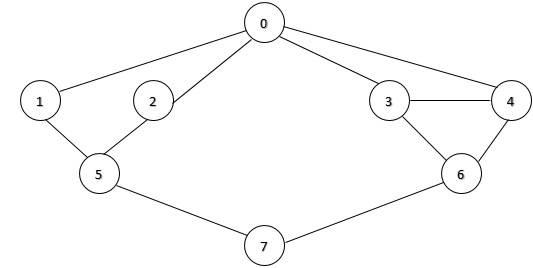
\includegraphics[width=12cm,height=6cm,keepaspectratio]{graph.png}    
\end{figure}
\begin{lstlisting}[language=C++]
#include <stdio.h>
#include <limits.h>
#define V 5
int minKey(int key[], bool mstSet[])
{
   int min = INT_MAX, min_index;
 
   for (int v = 0; v < V; v++)
     if (mstSet[v] == false && key[v] < min)
         min = key[v], min_index = v;
   return min_index;
}
int printMST(int parent[], int n, int graph[V][V])
{
   printf("Edge   Weight\n");
   for (int i = 1; i < V; i++)
      printf("%d - %d    %d \n", parent[i], i, graph[i][parent[i]]);
}
void primMST(int graph[V][V])
{
     int parent[V]; // Array to store constructed MST
     int key[V];   // Key values used to pick minimum weight edge in cut
     bool mstSet[V];  // To represent set of vertices not yet included in MST

     for (int i = 0; i < V; i++)
        key[i] = INT_MAX, mstSet[i] = false;
     key[0] = 0;     // Make key 0 so that this vertex is picked as first vertex
     parent[0] = -1;
     for (int count = 0; count < V-1; count++)
     {
        int u = minKey(key, mstSet);
        mstSet[u] = true;
        for (int v = 0; v < V; v++)
          if (graph[u][v] && mstSet[v] == false && graph[u][v] <  key[v])
             parent[v]  = u, key[v] = graph[u][v];
     }
     printMST(parent, V, graph);
}
int main()
{
   int graph[V][V] = {{0, 2, 0, 6, 0},
                      {2, 0, 3, 8, 5},
                      {0, 3, 0, 0, 7},
                      {6, 8, 0, 0, 9},
                      {0, 5, 7, 9, 0},
                     };
 
    // Print the solution
    primMST(graph);
 
    return 0;
}
\end{lstlisting}
 \textbf Output: Consider the Figure 1 for the output of the above code in the end of this document.

\textbf{Source Code} \\
https://goo.gl/ccBvqK

\begin{figure}[b!]
\centering
  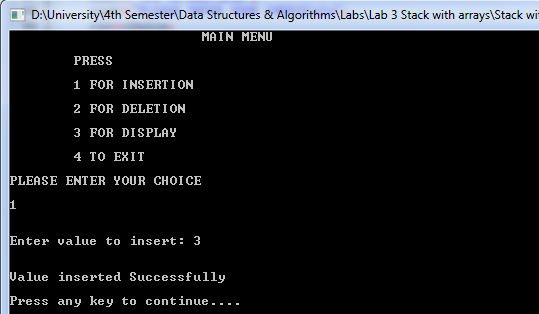
\includegraphics[width=12cm,height=6cm,keepaspectratio]{1.png}
\caption{Minimum Spanning Tree implementation on graph}
\label{Figure:1}    
\end{figure}

\section{Conclusion}
\justify Graphs are used to represent many real life applications: Graphs are used to represent networks. The networks may include paths in a city or telephone network or circuit network. Prim Minimum Spanning Tree algorithm can be implemented on graphs to visit every node in the shortest path, graphs may contain cycles, so we may come to the same node again. To avoid processing a node more than once, we use a boolean visited array.\\~\\

\tab[6cm] \noindent\rule{6cm}{0.4pt}\\
\tab[6cm] (Concerned Teacher/Lab Engineer)


 
\end{document}                          % The required last line
